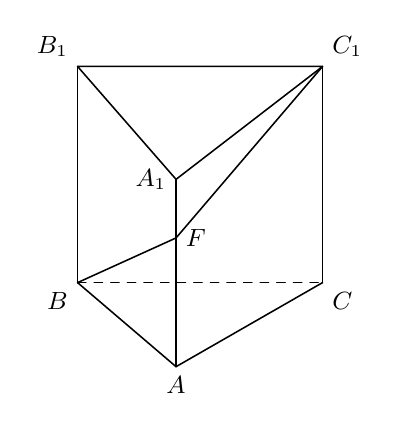
\begin{tikzpicture}[scale=.61, every node/.style={font=\small}, line cap=round, line join=round]
  \coordinate (B)  at (0,1.75);
  \coordinate (C)  at (5.10,1.75);
  \coordinate (A)  at (2.05,0);
  \coordinate (B1) at (0,6.25);
  \coordinate (C1) at (5.10,6.25);
  \coordinate (A1) at (2.05,3.90);
  \coordinate (F)  at (2.05,2.68);

  \draw[line width=.56pt] (B1)--(B) (C1)--(C) (A1)--(A);
  \draw[line width=.56pt] (B1)--(A1)--(C1)--cycle;
  \draw[line width=.56pt] (B)--(A)--(C);
  \draw[dashed, line width=.56pt] (B)--(C);
  \draw[line width=.56pt] (B)--(F)--(C1);

  \node[above left] at (B1) {$B_1$};
  \node[above right] at (C1) {$C_1$};
  \node[left] at (A1) {$A_1$};
  \node[below left] at (B) {$B$};
  \node[below right] at (C) {$C$};
  \node[below] at (A) {$A$};
  \node[right] at (F) {$F$};
\end{tikzpicture}
